{
\abnormalparskip{0pt}
\chapter{Discussion}
\label{cha:discussion}
}

This chapter discuss some of the observations made and obstacles met during the
work of the thesis.
% This includes elements which it would be wise to research more and elements which made

This chapter discusses some of the possible extension and directions for the
work of the thesis. 

\TODO[inline]{finish the introduction to the discussion}

\section{Observations and Obstacles}
\label{sec:observ-obst}

\TODO[inline]{}

\section{Possible Improvements}
\label{sec:poss-impr}

\TODO[inline]{}

\subsection{Concurrency}
\label{sec:concurrency}

Both the old and new implementation of the algorithm is implemented in a
sequential fashion. There also seems to be no literature concerned with making
the algorithm by \citeauthor{smith1992} concurrent.

Looking at \cref{fig:pprof} however may give an incitement to further
investigate the possibilities of making the algorithm concurrent. The figure
shows a CPU-time profile of the execution of the new implementation on a single
random instance (using the \citeauthor{smith1992}'s iteration for optimization).
As can be seen, more than $60\%$ of the elapsed time is spent in the function
which implements the iteration and above that the optimize function is more than
$80\%$ of the elapsed time. Making, especially the main loop concurrent, and
then run it in parallel on e.g.\ 4-8 CPUs (which is a very common amount of
CPUs in any modern desktop computer) could provide a very significant speed up.

\begin{figure}[htbp]
  \centering
  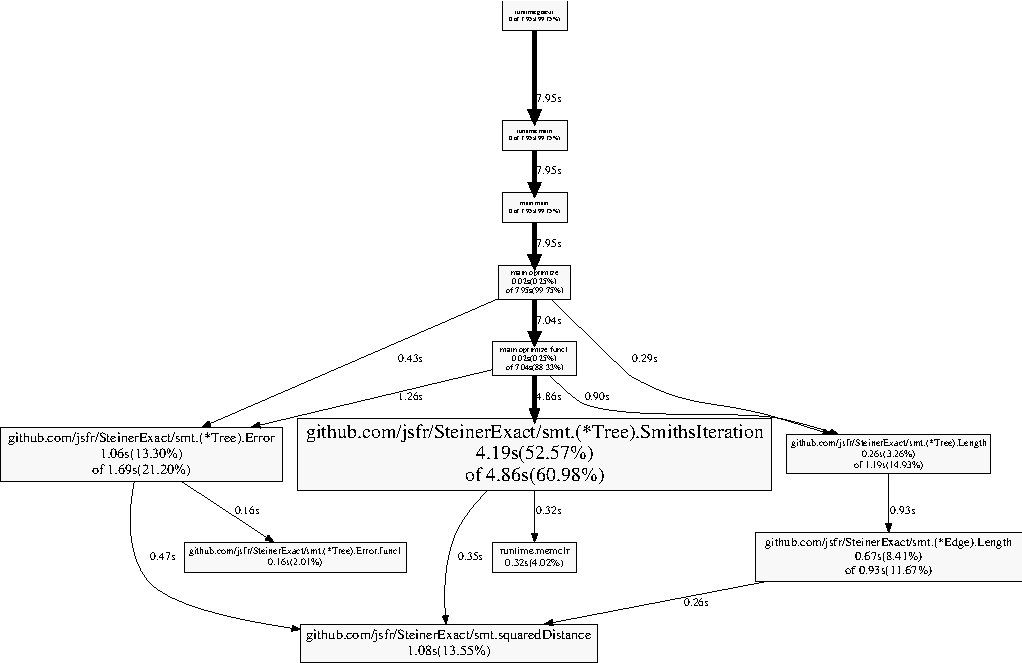
\includegraphics[width=\textwidth]{gfx/pprof001}
  \caption[CPU-time profile of a single execution]{CPU-time profile of the
    execution of the new implementation on a single random instance. The figure
    does not show the complete profile, as some of the smaller insignificant
    contributions have been remove for clarity.\label{fig:pprof}}
\end{figure}

The way one could make the algorithm concurrent would be to run the main loop of
the algorithm concurrently. We would then have to decide on some way of
splitting up the problem instances. One possible way of doing it would be to
start one process for each half of the children for the current topology vector.
So say we currently have the topology vector $[1, 2]$, we would then split this
into two new processes one which will look at $[1, 2, 1 \ldots 4]$ and one which looks
at $[1, 2, 5 \ldots 7]$. As long as we split in this fashion (no matter how many we
decide to split into) these can all be executed independently of each other, but
would of course benefit from synchronizing upper bounds. Thus we would make the
upper bound with a read-write lock which as mutual read (i.e.\ many can read the
upper bound at the same time) and exclusive write (i.e.\ only one can write a
new upper bound at a time). To avoid creating more processes than we have actual
CPUs we would probably also use a pool of workers.

Implementing a scheme as the one described above would allow us to both generate
and optimize multiple topology vectors in parallel which would provide a speedup
roughly equal to the number of CPUs we have available. However this approach
would also allow us to find upper bounds in parallel, which could mean that
topologies which we before were not able to prune, will now be pruned. Thus the
shared upper bound between processes could result in a further speedup.

The new implementation is as mentioned written in Go, which is a language that
makes concurrency very straightforward. Thus extending the new implementation to
use concurrency could be done by just refactoring a slightly changed version of
the main loop to a new function, and then spawn new goroutines. These should
then e.g.\ have a topology vector and some some boundaries for which part of the
descendants it should generate. Due to Go's way of making arrays, we would also
need to expand the \texttt{Tree} struct with a new function to clone the tree.
This would result in a slight slowdown, but more importantly it would require
the more memory equivalent again approximately to the number of running
processes.

\subsection{Lower Bounds and Geometric Properties}
\label{sec:lower-bounds-geom}

As is also proposed in \textcite{fonseca2014} one could also try to apply either
the lower bounds proposed in \textcite{fampa2008} a
Lower bounds? these however seem to all be very complex.

\subsection{Propagating Changes in the Simple Iteration}
\label{sec:prop-chang-simple}

Lad analytisk metode propagerer sine changes ud fra nyt steiner punkt, og
evt. tilbage igen

Kører iteration kun på den del der er blevet ændret, dvs. kun de FSTs der er
affekteret af det fulde FST.

\subsection{Initial Placement of Steiner Points}
\label{sec:init-plac-stein}

Currently both the old and new implementation place the Steiner points at the
perturbed centroid of their neighbors. However the calculating the centroid is
about as computationally heavy, as using calculating the Fermat-Torricelli point
using the analytical solution. Thus the implementation would probably benefit
from exchanging the perturbed centroid with the perturbed Fermat-Torricelli
point as a initial placement. The reasoning behind this, is that all Steiner
points will be closer to their final optimal coordinates and thus we would need
fewer iterations in total.

\begin{table}[htbp]
  \centering
  \begin{tabular}{ccccccc}
    \toprule
         & \multicolumn{2}{c}{\footnotesize{\textit{Centroid}}}
         & \multicolumn{2}{c}{\footnotesize{\textit{Fermat-Torricelli point}}}
         & \multicolumn{2}{c}{\footnotesize{\textit{Ratio}}}                     \\
    $n$  & Iterations & Trees     & Iterations & Trees     & Iterations & Trees  \\
    \cmidrule(r){1-1}\cmidrule(lr){2-3}\cmidrule(lr){4-5}\cmidrule(l){6-7}
    $10$ & $73132.7$  & $4231.94$ & $58443.5$  & $1645.08$ & $0.80$     & $0.39$ \\ 
    $11$ & $307128$   & $18429$   & $238776$   & $6944.14$ & $0.78$     & $0.38$ \\
    $12$ & $1492050$  & $87869.2$ & $1122520$  & $32192.1$ & $0.75$     & $0.37$ \\
    \bottomrule
  \end{tabular}
  \caption[Perturbed centroid vs.\ perturbed Fermat-Torricelli point]{The table shows the average number of trees optimized and
    number of optimization iterations when placing the Steiner points at the perturbed
    centroid or the perturbed Fermat-Torricelli point initially. The data is for
    the cube instances used in \cref{sec:correctness}. \citeauthor{smith1992}'s iteration without terminal sorting was used. The last two columns
    show the ratio between the numbers for easier comparison. There are $50$
    instances of for each $n$.\label{tab:centroid-vs-fermat}}
\end{table}

To test the potential impact of this change a quick test was performed were the
use of the perturbed centroid was exchanged with the Fermat-Torricelli point,
perturbed exactly the same amount as the centroid was. The cube instances from
\cref{sec:correctness} were then run before and after the change, and the
average for the number of trees optimized and iterations for $n=10,11,12$ were
calculated. The results can be found in \cref{tab:centroid-vs-fermat}. The data
is only for running \citeauthor{smith1992}'s iteration (without terminal
sorting) to be sure that the data is not affected by the sub-optimality seen in
\cref{sec:correctness} for the simple iteration\footnote{Furthermore the
  correctness test were performed again after the change just for good measure.
  This showed no new sub-optimal results, apart from those in the simple
  iteration already known.}. As can be seen, at least for this data set, the
program ran $\approx 20\%$ fewer iterations, and optimized $\approx 60\%$ fewer
trees. It therefore seems worthwhile to make this very simple change, but more
extensive performance tests would probably have to be made.

%%% Local Variables:
%%% mode: latex
%%% TeX-master: "../../main"
%%% End:
